\documentclass[12pt]{article}

\usepackage{amsmath}
\usepackage{amssymb}
\usepackage[dvips]{graphicx}
%\usepackage{lscape}
\usepackage{eepic}
\usepackage{color}
\usepackage{wasysym} % \female \male
\usepackage[landscape,pdftex]{geometry}
\usepackage{fancyhdr}
\usepackage{hyperref}

\definecolor{cantelope}{rgb}{1.0,0.8,0.4}
\hypersetup{
    colorlinks, urlcolor={cantelope}
}
\hypersetup{pdfpagemode=UseNone} % don't show bookmarks on initial view

\DeclareOption{bigsym}{\DeclareSymbolFont{largesymbols}{OMX}{psycm}{m}{n}}
\ProcessOptions

\setlength{\oddsidemargin}{-0.75in}
\setlength{\evensidemargin}{-0.75in}
\setlength{\topmargin}{-1in}
\setlength{\textheight}{7.75in}
\setlength{\textwidth}{10.5in}
\setlength{\footskip}{0in}
\setlength{\parindent}{0pt}
\setlength{\rightskip}{0pt plus 1fil} % makes ragged right

\renewcommand{\familydefault}{phv} % helvetica

% following: color
\definecolor{mybgcolor}{rgb}{0,0,0.3125}
\definecolor{myyellow}{rgb}{1,1,0.4}
\definecolor{myblue}{rgb}{0.4,0.8,1}
\definecolor{mypink}{rgb}{1,0.4,1}
\definecolor{mywhite}{rgb}{1,1,1}

% following: B/W
%\definecolor{mybgcolor}{rgb}{1,1,1}
%\definecolor{myyellow}{rgb}{0,0,0}
%\definecolor{myblue}{rgb}{0,0,0}
%\definecolor{mypink}{rgb}{0,0,0}
%\definecolor{mywhite}{rgb}{0,0,0}

% header/footer layout
\pagestyle{fancy}
\lhead{} \chead{} \rhead{}
\lfoot{} \cfoot{} \rfoot{\color{myyellow} \thepage}
\renewcommand{\headrulewidth}{0pt}
\renewcommand{\footrulewidth}{0pt}

% font sizes
\newcommand{\superlarge}{\fontsize{60}{60} \selectfont}
\newcommand{\titlesize}{\fontsize{40}{50} \selectfont}
\newcommand{\headsize}{\fontsize{35}{35} \selectfont}
\newcommand{\textsize}{\fontsize{30}{35} \selectfont}
\newcommand{\smallsize}{\fontsize{25}{30} \selectfont}
\newcommand{\smallersize}{\fontsize{20}{25} \selectfont}
\newcommand{\smallestsize}{\fontsize{18}{22} \selectfont}
\newcommand{\lod}{\text{LOD}}
\newcommand{\rss}{\text{RSS}}
\newcommand{\var}{\text{var}}
\newcommand{\M}{\text{M}}
%\renewcommand{\log}{\text{log}}
%\renewcommand{\max}{\text{max}}



\pagecolor{mybgcolor}
\color{mywhite}

\begin{document}

\begin{center}
\titlesize \color{myyellow}

\vspace*{3cm}

QTL mapping \\
in experimental crosses \\[24pt]
{\color{mywhite} Part I}
\end{center}

\vfill


\hfill \begin{minipage}{5in}
\color{myblue}  \smallsize
Karl W Broman \\
\smallersize
\href{http://kbroman.org}{\tt kbroman.org} \\
\href{https://github.com/kbroman}{\tt github.com/kbroman} \\
\href{https://twitter.com/kwbroman}{\tt @kwbroman}


\vspace{10mm}



\vspace{10mm}

\end{minipage}





\newpage
\thispagestyle{empty}

\vspace*{-0.85in}

\centerline{\includegraphics[height=9in]{Figs/inbredmice.jpg}}


\newpage

\headsize \color{myyellow}
\hfill \begin{minipage}{5.75in}
\centering
Human vs mouse
\end{minipage}

\vspace{3cm}

\centerline{
\includegraphics[height=5in]{Figs/da-vinci-man.jpg}
\includegraphics[height=5in]{Figs/vitruvian_mouse.jpg}
}

{\color{myblue} \smallestsize \hfill
  \href{http://www.daviddeen.com}{\tt www.daviddeen.com} \hspace*{11mm}}


\newpage

\headsize \color{myyellow}
\hfill \begin{minipage}{5.75in}
\centering
Backcross
\end{minipage}

\vfill

\centerline{\includegraphics{Figs/backcross.pdf}}

\newpage

\headsize \color{myyellow}
\hfill \begin{minipage}{5.75in}
\centering
Intercross
\end{minipage}

\vfill

\centerline{\includegraphics{Figs/intercross.pdf}}

\newpage

\headsize \color{myyellow}
\hfill \begin{minipage}{5.75in}
\centering
Meiosis
\end{minipage}

\vfill

\centerline{\includegraphics[height=6.5in]{Figs/meiosis.png}}

\vspace{10mm}

\newpage

\headsize \color{myyellow}
\hfill \begin{minipage}{5.75in}
\centering
Genetic distance
\end{minipage}

\vspace{3cm}

\smallsize \color{mywhite}
\hfill \begin{minipage}{9.5in}

\begin{itemize}
\itemsep18pt
\item Genetic distance between two markers (in cM) =

\vspace{18pt}

\hspace*{2cm}
\begin{minipage}{7in}
\setlength{\rightskip}{0pt plus 1fil} % makes ragged right

{\color{mypink} Average number of crossovers in the interval in 100
  meiotic products.}
\end{minipage}

\item ``Intensity'' of the crossover point process

\item Recombination rate varies by

\begin{itemize}
\smallersize
\color{myblue}
\itemsep6pt
\item Organism
\item Sex
\item Chromosome
\item Position on chromosome
\end{itemize}

\end{itemize}
\end{minipage}


\newpage


\headsize \color{myyellow}
\hfill \begin{minipage}{5.75in}
\centering
Recombination fraction
\end{minipage}

\vspace{3cm}

\begin{minipage}{6in}
\vspace*{0pt}

\includegraphics[width=6in]{Figs/recombination.jpg}
\end{minipage} \hfill
\begin{minipage}{4in}
\vspace*{5mm}
\smallestsize
\color{mywhite}
\setlength{\rightskip}{0pt plus 1fil} % makes ragged right

We generally do not observe the locations of crossovers; rather, we
observe the grandparental origin of DNA at a set of {\color{mypink}
  genetic markers}.

\vspace{1cm}

{\color{mypink} Recombination} across an interval indicates an
{\color{mypink} odd} number of crossovers.
\end{minipage}


\vspace{25mm}

\smallsize

{\color{mypink} Recombination fraction = }

\vspace{5mm}

\hfill {\color{myblue} Pr(recombination in interval) = Pr(odd
  no. XOs in interval)}



\newpage

\headsize \color{myyellow}
\hfill \begin{minipage}{5.75in}
\centering
Map functions
\end{minipage}

\vspace{3cm}

\smallersize \color{mywhite}
\hfill \begin{minipage}{9.5in}

\begin{itemize}
\setlength{\rightskip}{0pt plus 1fil} % makes ragged right
\itemsep18pt
\item A map function relates the {\color{mypink} genetic length} of an
  interval and the {\color{mypink} recombination fraction}.

\vspace{18pt}

\centerline{
\begin{minipage}{3in}
{\color{mypink} r = M(d) }
\end{minipage}  }

\item Map functions are related to {\color{mypink} crossover interference}, but a map
  function is not sufficient to define the crossover process.

\item Haldane map function{\color{myblue} : no crossover interference}

\item Kosambi{\color{myblue} : similar to the level of interference
  in humans}

\item Carter-Falconer{\color{myblue} : similar to the level of
  interference in mice}
\end{itemize} \end{minipage}



\newpage

\headsize \color{myyellow}
\hfill \begin{minipage}{5.75in}
\centering
Intercross
\end{minipage}

\vfill

\centerline{\includegraphics{Figs/intercross.pdf}}



\newpage

\headsize \color{myyellow}
\hfill \begin{minipage}{5.75in}
\centering
Phenotype data
\end{minipage}

\vspace{30mm}

\centerline{\includegraphics{Figs/pheno.pdf}}

\vfill
\smallestsize
\color{myblue}
Sugiyama et al.\ (2002) Physiol Genomics 10:5--12


\newpage

\headsize \color{myyellow}
\hfill \begin{minipage}{5.75in}
\centering
Genetic map
\end{minipage}

\vfill

\centerline{\includegraphics{Figs/geneticmap.pdf}}

\newpage

\headsize \color{myyellow}
\hfill \begin{minipage}{5.75in}
\centering
Genotype data
\end{minipage}

\vfill

\centerline{\includegraphics{Figs/genodata.pdf}}


\newpage

\headsize \color{myyellow}
\hfill \begin{minipage}{5.75in}
\centering
Goals
\end{minipage}

\vspace{3cm}

\color{mywhite} \smallsize

\hfill \begin{minipage}[t]{9.5in}
\begin{itemize}
\itemsep24pt
\item Identify quantitative trait loci (QTL)\\[6pt]
   {\color{myblue}   (and interactions among QTL)}
\item Interval estimates of QTL location
\item Estimated QTL effects
\end{itemize} \end{minipage}


\newpage

\headsize \color{myyellow}
\hfill \begin{minipage}{5.75in}
\centering
Statistical structure
\end{minipage}

\vspace{2cm} \color{mywhite} \smallersize

\centerline{\includegraphics{Figs/structure.pdf}}

\vspace{15mm}

\hspace*{3cm}\begin{tabular}{lll}
{\color{mypink} The missing data problem:}  & \hspace{15mm} &
Markers $\longleftrightarrow$ QTL \\[15mm]

{\color{mypink} The model selection problem:}
& & QTL, covariates $\longrightarrow$ phenotype
\end{tabular}





\newpage

\headsize \color{myyellow}
\hfill\begin{minipage}{5.75in}
\centering
ANOVA at marker loci
\end{minipage}

\vspace{2cm}

\color{mywhite} \smallsize

\hspace*{0.5in}
\begin{minipage}[t]{4.1in}
\vspace*{5mm}

\sloppy
\smallersize
\begin{itemize}
\setlength{\rightskip}{0pt plus 1fil} % makes ragged right
\item Also known as {\color{mypink} marker regression}.
\item Split mice into groups according to genotype at a marker.
\item Do a t-test / ANOVA.
\item Repeat for each marker.
\end{itemize}
\end{minipage}
\hfill
\begin{minipage}[t]{5.3in}
\vspace*{0mm}

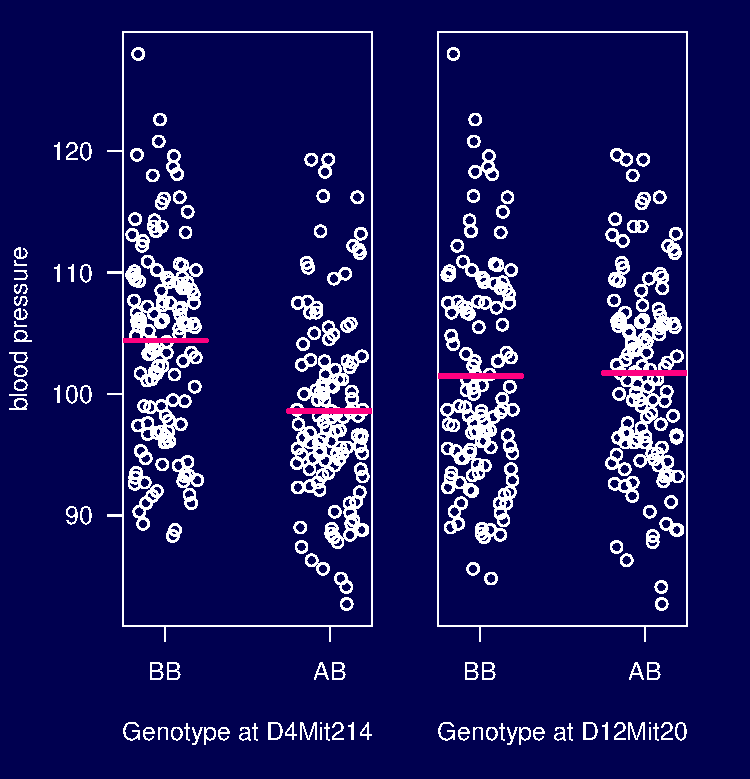
\includegraphics{Figs/anova.pdf}
\end{minipage}







\newpage

\headsize \color{myyellow}
\hfill \begin{minipage}{5.75in}
\centering
ANOVA at marker loci
\end{minipage}

\vspace{2cm}

\color{mywhite} \smallsize

\hspace*{0.5in}
\begin{minipage}[t]{4.8in}
\textsize {\color{mypink} Advantages}

\smallersize \color{mywhite}
\begin{itemize}
\setlength{\rightskip}{0pt plus 1fil} % makes ragged right
\item Simple.
\item Easily incorporates covariates.
\item Easily extended to more complex models.
\item Doesn't require a genetic map.
\end{itemize}
\end{minipage}
\hfill
\begin{minipage}[t]{4.8in}
\textsize {\color{mypink} Disadvantages}

\smallersize \color{mywhite}
\begin{itemize}
\setlength{\rightskip}{0pt plus 1fil} % makes ragged right
\item Must exclude individuals with missing genotype data.
\item Imperfect information about QTL location.
\item Suffers in low density scans.
\item {\color{mypink} Only considers one QTL at a time.}
\end{itemize}
\end{minipage}






\newpage

\headsize \color{myyellow}
\hfill \begin{minipage}{5.75in}
\centering
Interval mapping
\end{minipage}

\vspace{15mm}

\hspace*{0.5in}
\color{mywhite} \smallsize
Lander \& Botstein (1989)
\vspace{1cm}

\smallersize
\hfill \begin{minipage}{9.5in}
\begin{itemize}
\itemsep24pt
\setlength{\rightskip}{0pt plus 1fil} % makes ragged right
  \item Assume a {\color{mypink} single} QTL model.
  \item Each position in the genome, one at a time, is posited as the
  putative QTL.
  \item Let $\mathsf{q = }$ 1/0 if the (unobserved) QTL genotype is
  BB/AB. \\[12pt]
  {\color{myblue} (Or 2/1/0 if the QTL genotype is BB/AB/AA in an intercross.)} \\[12pt]
        Assume $\mathsf{y | q \sim N(\mu_q, \sigma)}$
  \item Given genotypes at linked markers, $\mathsf{y \sim}$ mixture of normal
  dist'ns with mixing proportions $\mathsf{\Pr(q \ | \ \text{marker data})}$
\end{itemize}
\end{minipage}
\newpage

\headsize \color{myyellow}
\hfill \begin{minipage}{5.75in}
\centering
Genotype probabilities
\end{minipage}

\vspace{15mm}

\centerline{\includegraphics{Figs/genoprob1.pdf}}

\vspace{15mm}

\hfill
\begin{minipage}{10in}
\color{mywhite} \smallersize
Calculate {\color{myblue} $\mathsf{\Pr(q \ | \ \text{marker data})}$}, assuming
\begin{itemize}
\item No crossover interference
\item No genotyping errors
\end{itemize}

\vspace{10mm}

Or use the {\color{mypink} hidden Markov model (HMM)} technology
\begin{itemize}
\item To allow for genotyping errors
\item To incorporate dominant markers
\item {\color{myblue} (Still assume no crossover interference.)}
\end{itemize}
\end{minipage}



\newpage

\addtocounter{page}{-1}

\headsize \color{myyellow}
\hfill \begin{minipage}{5.75in}
\centering
Genotype probabilities
\end{minipage}

\vspace{15mm}

\centerline{\includegraphics{Figs/genoprob2.pdf}}

\vspace{15mm}

\hfill
\begin{minipage}{10in}
\color{mywhite} \smallersize
Calculate {\color{myblue} $\mathsf{\Pr(q \ | \ \text{marker data})}$}, assuming
\begin{itemize}
\item No crossover interference
\item No genotyping errors
\end{itemize}

\vspace{10mm}

Or use the {\color{mypink} hidden Markov model (HMM)} technology
\begin{itemize}
\item To allow for genotyping errors
\item To incorporate dominant markers
\item {\color{myblue} (Still assume no crossover interference.)}
\end{itemize}
\end{minipage}

\newpage

\addtocounter{page}{-1}

\headsize \color{myyellow}
\hfill \begin{minipage}{5.75in}
\centering
Genotype probabilities
\end{minipage}

\vspace{15mm}

\centerline{\includegraphics{Figs/genoprob3.pdf}}

\vspace{15mm}

\hfill
\begin{minipage}{10in}
\color{mywhite} \smallersize
Calculate {\color{myblue} $\mathsf{\Pr(q \ | \ \text{marker data})}$}, assuming
\begin{itemize}
\item No crossover interference
\item No genotyping errors
\end{itemize}

\vspace{10mm}

Or use the {\color{mypink} hidden Markov model (HMM)} technology
\begin{itemize}
\item To allow for genotyping errors
\item To incorporate dominant markers
\item {\color{myblue} (Still assume no crossover interference.)}
\end{itemize}
\end{minipage}


\newpage

\addtocounter{page}{-1}

\headsize \color{myyellow}
\hfill \begin{minipage}{5.75in}
\centering
Genotype probabilities
\end{minipage}

\vspace{15mm}

\centerline{\includegraphics{Figs/genoprob4.pdf}}

\vspace{15mm}

\hfill
\begin{minipage}{10in}
\color{mywhite} \smallersize
Calculate {\color{myblue} $\mathsf{\Pr(q \ | \ \text{marker data})}$}, assuming
\begin{itemize}
\item No crossover interference
\item No genotyping errors
\end{itemize}

\vspace{10mm}

Or use the {\color{mypink} hidden Markov model (HMM)} technology
\begin{itemize}
\item To allow for genotyping errors
\item To incorporate dominant markers
\item {\color{myblue} (Still assume no crossover interference.)}
\end{itemize}
\end{minipage}


\newpage

\addtocounter{page}{-1}

\headsize \color{myyellow}
\hfill \begin{minipage}{5.75in}
\centering
Genotype probabilities
\end{minipage}

\vspace{15mm}

\centerline{\includegraphics{Figs/genoprob5.pdf}}

\vspace{15mm}

\hfill
\begin{minipage}{10in}
\color{mywhite} \smallersize
Calculate {\color{myblue} $\mathsf{\Pr(q \ | \ \text{marker data})}$}, assuming
\begin{itemize}
\item No crossover interference
\item No genotyping errors
\end{itemize}

\vspace{10mm}

Or use the {\color{mypink} hidden Markov model (HMM)} technology
\begin{itemize}
\item To allow for genotyping errors
\item To incorporate dominant markers
\item {\color{myblue} (Still assume no crossover interference.)}
\end{itemize}
\end{minipage}


\newpage

\addtocounter{page}{-1}

\headsize \color{myyellow}
\hfill \begin{minipage}{5.75in}
\centering
Genotype probabilities
\end{minipage}

\vspace{15mm}

\centerline{\includegraphics{Figs/genoprob6.pdf}}

\vspace{15mm}

\hfill
\begin{minipage}{10in}
\color{mywhite} \smallersize
Calculate {\color{myblue} $\mathsf{\Pr(q \ | \ \text{marker data})}$}, assuming
\begin{itemize}
\item No crossover interference
\item No genotyping errors
\end{itemize}

\vspace{10mm}

Or use the {\color{mypink} hidden Markov model (HMM)} technology
\begin{itemize}
\item To allow for genotyping errors
\item To incorporate dominant markers
\item {\color{myblue} (Still assume no crossover interference.)}
\end{itemize}
\end{minipage}




\newpage

\headsize \color{myyellow}
\hfill \begin{minipage}{5.75in}
\centering
The normal mixtures
\end{minipage}

\vspace{15mm}

\hspace*{0.5in}
\begin{minipage}[t]{4.6in}
\vspace*{10mm}

\color{mywhite} \smallersize
\setlength{\unitlength}{1.0in}
\begin{center}
\begin{picture}(4.5,1)
% lines
\Thicklines
\put(0.25,0.5){\line(1,0){4}}
\put(0.25,0.35){\line(0,1){0.3}}
\put(1.65,0.35){\line(0,1){0.3}}
\put(4.25,0.35){\line(0,1){0.3}}

% text
\put(0.25,0.1){\makebox(0,0){$\mathsf{M_1}$}}
\put(4.25,0.1){\makebox(0,0){$\mathsf{M_2}$}}
\put(1.65,0.1){\makebox(0,0){$\mathsf{Q}$}}
\put(0.95,0.8){\makebox(0,0){7 cM}}
\put(2.95,0.8){\makebox(0,0){13 cM}}
\end{picture} \end{center}
\vspace{5mm}

\begin{itemize}
\setlength{\rightskip}{0pt plus 1fil} % makes ragged right
\item Two markers separated by 20 cM, with the QTL closer to the left marker.
\item The figure at right shows the distributions of the phenotype
conditional on the genotypes at the two markers.
\item The dashed curves correspond to the components of the mixtures.
\end{itemize}

\end{minipage}
\hfill
\begin{minipage}[t]{4.6in}
\vspace*{0mm}

\includegraphics{Figs/mixtures.pdf}
\end{minipage}




\newpage

\headsize \color{myyellow}
\hfill \begin{minipage}{5.75in}
\centering
Interval mapping
\end{minipage}

\vspace{25mm}

\hfill \begin{minipage}{10in}
\color{mywhite} \smallsize
 Let $\mathsf{p_{ij} = \Pr(q_i = j | \text{marker data})}$
\vspace{10mm}

 $\mathsf{y_i | q_i \sim N(\mu_{q_i},\sigma^2)}$
\vspace{10mm}

 $\mathsf{\Pr(y_i | \text{marker data},\mu_0,\mu_1,\sigma) =
\sum_j p_{ij} \, f(y_i; \mu_j,\sigma)}$
\vspace{10mm}

\hspace{15mm} where $\mathsf{f(y; \mu,\sigma)= \exp[-(y-\mu)^2/(2\sigma^2)] / \sqrt{2 \pi
\sigma^2}}$
\vspace{15mm}

 {\color{mypink} Log likelihood}: \hspace{5mm}
$\mathsf{l(\mu_0,\mu_1,\sigma) = \sum_i \log \Pr(y_i | \text{marker
data},\mu_0,\mu_1,\sigma)}$
\vspace{10mm}

 Maximum likelihood estimates ({\color{mypink} MLEs})
of $\mathsf{\mu_0}$, $\mathsf{\mu_1}$, $\mathsf{\sigma}$:
\vspace{5mm}

\hspace{15mm} values for which $\mathsf{l(\mu_0,\mu_1,\sigma)}$ is maximized.
\end{minipage}

\newpage

\headsize \color{myyellow}
\hfill \begin{minipage}{5.75in}
\centering
EM algorithm
\end{minipage}

\vspace{15mm}

\hfill
\begin{minipage}{10in}
\color{mywhite} \smallsize
 Dempster et al.\ (1977)
\vspace{5mm}

 {\color{mypink} E step}:
\vspace{5mm}

\hspace{10mm} Let \hspace{5mm} $\mathsf{w_{ij}^{(k)} = \Pr(q_i = j | y_i,\text{marker
data},\hat{\mu}_0^{(k-1)}, \hat{\mu}_1^{(k-1)},\hat{\sigma}^{(k-1)})}$
\vspace{5mm}

\hspace{56mm} $\mathsf{ = \frac{p_{ij} \,
f(y_i; \hat{\mu}_j^{(k-1)},\hat{\sigma}^{(k-1)})}{
\sum_j p_{ij} \, f(y_i; \hat{\mu}_j^{(k-1)},\hat{\sigma}^{(k-1)})}}$
\vspace{5mm}

 {\color{mypink} M step}:
\vspace{5mm}

\hspace{10mm} Let \hspace{5mm} $\mathsf{\hat{\mu}_j^{(k)} = \sum_i y_i w_{ij}^{(k)} / \sum_i
w_{ij}^{(k)}}$
\vspace{5mm}

\hspace{31.5mm} $\mathsf{\hat{\sigma}^{(k)} = \sqrt{ \sum_i \sum_j w_{ij}^{(k)}
(y_i-\hat{\mu}_j^{(k)})^2/n}}$
\vspace{5mm}

 {\color{mypink} The algorithm}:
\vspace{5mm}

\hspace{10mm} Start with $\mathsf{w_{ij}^{(1)} = p_{ij}}$; iterate the E \& M steps until
convergence.
\end{minipage}

\newpage

\headsize \color{myyellow}
\hfill \begin{minipage}{5.75in}
\centering
LOD scores
\end{minipage}

\vspace{25mm}

\hfill
\begin{minipage}{10in}
\color{mywhite} \smallersize
 The LOD score is a measure of the {\color{mypink} strength of
evidence} for the presence of a QTL at a particular
location.
\vspace{15mm}

 $\mathsf{\lod(\lambda)}$
\begin{minipage}[t]{8.5in}
$\mathsf{= \log_{10}}$ likelihood ratio comparing the hypothesis of a \\
\hspace*{8mm} QTL at position $\mathsf{\lambda}$ versus that of no QTL
\vspace{5mm}

\headsize
$\mathsf{= \log_{10} \left\{ \frac{\Pr(y | \text{QTL at $\lambda$}, \hat{\mu}_{0\lambda},
\hat{\mu}_{1\lambda}, \hat{\sigma}_\lambda)}{\Pr(y | \text{no QTL}, \hat{\mu},
\hat{\sigma})} \right\}}$
\end{minipage}
\vspace{15mm}

 $\mathsf{\hat{\mu}_{0\lambda}, \hat{\mu}_{1\lambda}, \hat{\sigma}_\lambda}$ are the MLEs,
assuming a single QTL at position $\mathsf{\lambda}$.
\vspace{15mm}

 No QTL model:
\begin{minipage}[t]{7.5in}
The phenotypes are independent and identically
distributed (iid) $\mathsf{N(\mu, \sigma^2)}$.
\end{minipage}
\end{minipage}







\newpage

\headsize \color{myyellow}
\hfill \begin{minipage}{5.75in}
\centering
LOD curves
\end{minipage}

\vfill

\centerline{\includegraphics{Figs/alod.pdf}}



\newpage

\headsize \color{myyellow}
\hfill \begin{minipage}{5.75in}
\centering
\href{http://www.biostat.wisc.edu/~kbroman/D3/lod_and_effect/}{Interactive plot}
\end{minipage}

\vfill

\centerline{\href{http://www.biostat.wisc.edu/~kbroman/D3/lod_and_effect/}{\includegraphics[height=6.5in]{Figs/interactive_lod_curve.png}}}

\vspace*{1cm}






\newpage

\headsize \color{myyellow}
\hfill \begin{minipage}{5.75in}
\centering
Interval mapping
\end{minipage}

\vspace{2cm}

\color{mywhite} \smallsize

\hspace*{0.5in}
\begin{minipage}[t]{4.8in}
\textsize {\color{mypink} Advantages}

\smallersize \color{mywhite}
\begin{itemize}
\setlength{\rightskip}{0pt plus 1fil} % makes ragged right
\item Takes proper account of missing data.
\item Allows examination of positions between markers.
\item Gives improved estimates of QTL effects.
\item Provides pretty graphs.
\end{itemize}
\end{minipage}
\hfill
\begin{minipage}[t]{4.8in}
\textsize {\color{mypink} Disadvantages}

\smallersize \color{mywhite}
\begin{itemize}
\setlength{\rightskip}{0pt plus 1fil} % makes ragged right
\item Increased computation time.
\item Requires specialized software.
\item Difficult to generalize.
\item {\color{mypink} Only considers one QTL at a time.}
\end{itemize}
\end{minipage}




\newpage

\headsize \color{myyellow}
\hfill \begin{minipage}{5.75in}
\centering
LOD thresholds
\end{minipage}

\smallersize \color{mywhite}

\vspace{25mm}

\hfill
\begin{minipage}{10in}
Large LOD scores indicate evidence for the presence of a QTL
\vspace{5mm}

{\color{mypink} Question}: How large is large?
\vspace{20mm}

{\color{myyellow} LOD threshold} =  \hspace{2mm}
\begin{minipage}[t]{7in}
\setlength{\rightskip}{0pt plus 1fil} % makes ragged right
95 \%ile of distr'n of max LOD, genome-wide, if there are no QTLs anywhere
\end{minipage}
\vspace{20mm}

\hspace{15mm} {\color{myyellow} Derivation:} \hfill
\begin{minipage}[t]{7.5in}
\begin{itemize}
\item Analytical calculations (L \& B 1989)
\item Simulations (L \& B 1989)
\item Permutation tests (Churchill \& Doerge 1994)
\end{itemize} \end{minipage}
\end{minipage}



\newpage

\headsize \color{myyellow}
\hfill \begin{minipage}{5.75in}
\centering
Null distribution of the LOD score
\end{minipage}

\vspace{3cm}

\hspace*{0.5in}
\begin{minipage}[t]{4.7in}
\vspace*{10mm}

\color{mywhite} \smallersize
\begin{itemize}
\setlength{\rightskip}{0pt plus 1fil} % makes ragged right
\item Null distribution derived by computer simulation of backcross
with genome of typical size.
\item Dashed curve: distribution of LOD score at any one point.
\item Solid curve: distribution of maximum LOD score, genome-wide.
\end{itemize}
\end{minipage}
\hfill
\begin{minipage}[t]{4.7in}
\vspace*{0cm}

\includegraphics{Figs/loddist.pdf}
\end{minipage}








\newpage

\headsize \color{myyellow}
\hfill \begin{minipage}{5.75in}
\centering
Permutation test
\end{minipage}

\vspace{2cm}

\centerline{\includegraphics{Figs/permtest.pdf}}

\newpage

\headsize \color{myyellow}
\hfill \begin{minipage}{5.75in}
\centering
Permutation results
\end{minipage}

\vfill

\centerline{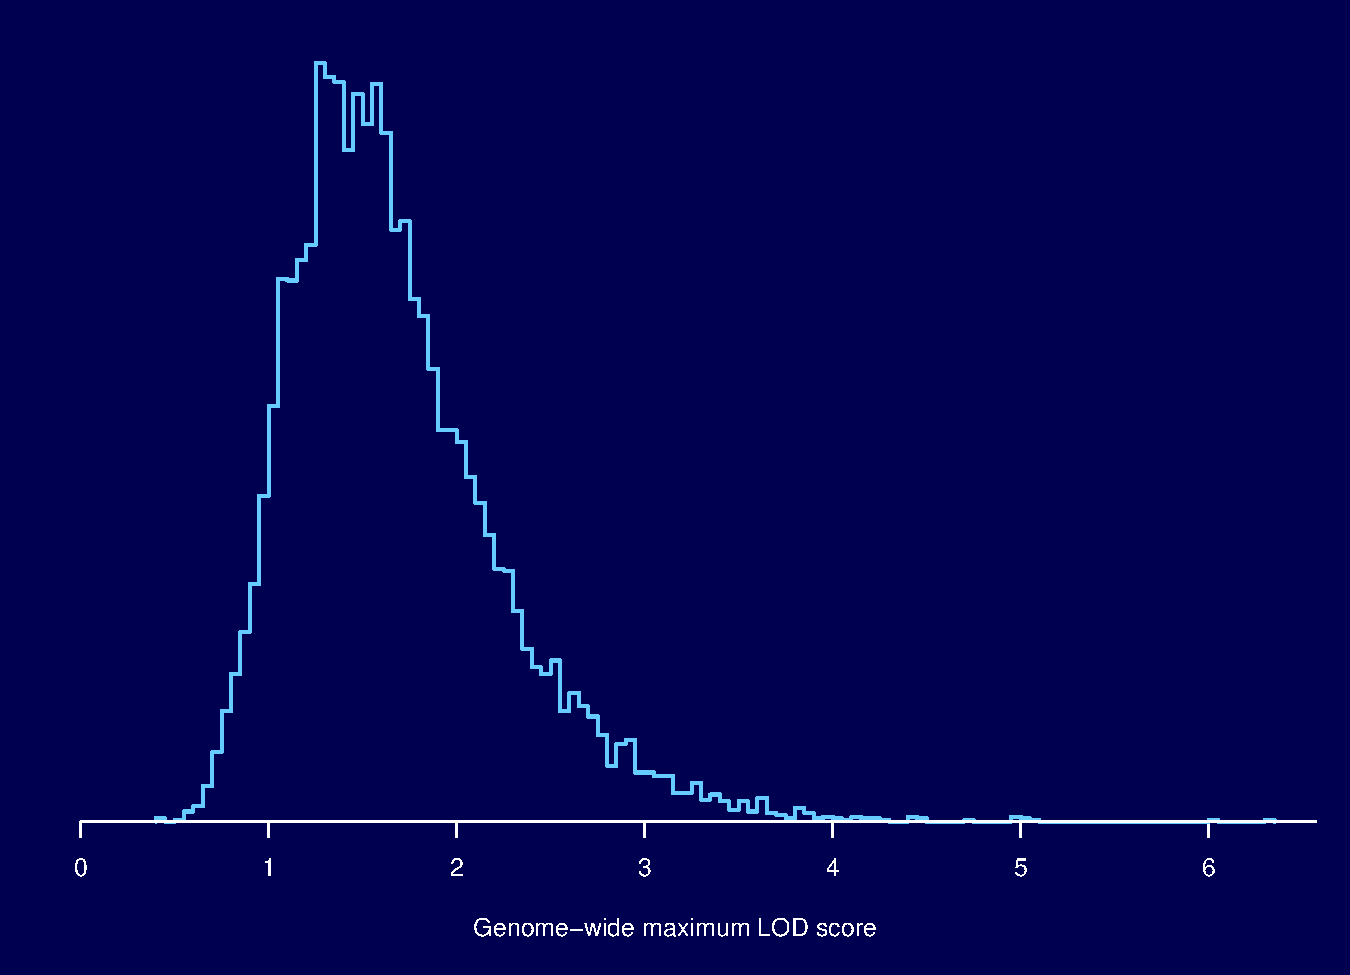
\includegraphics{Figs/perm_hist.pdf}}



\newpage

\headsize \color{myyellow}
\hfill \begin{minipage}{5.75in}
\centering
LOD curves
\end{minipage}

\vfill

\centerline{\includegraphics{Figs/alod.pdf}}


\newpage

\headsize \color{myyellow}
\hfill \begin{minipage}{5.75in}
\centering
\href{http://www.biostat.wisc.edu/~kbroman/D3/lod_random/}{Interactive plot}
\end{minipage}

\vspace{2cm}

\centerline{\href{http://www.biostat.wisc.edu/~kbroman/D3/lod_random}{\includegraphics[width=10in]{Figs/interactive_perm_test.png}}}

\vspace*{1cm}




\newpage

\headsize \color{myyellow}
\hfill \begin{minipage}{5.75in}
\centering
LOD support intervals
\end{minipage}

\vfill

\centerline{\includegraphics{Figs/lodsuppint.pdf}}






\newpage

\headsize \color{myyellow}
\hfill \begin{minipage}{5.75in}
\centering
Modelling multiple QTL
\end{minipage}

\vspace{2cm}

\color{mywhite} \smallsize

\hfill \begin{minipage}[t]{10in}
\begin{itemize}
\itemsep24pt
\item Reduce residual variation $\implies$ increased power

\item Separate linked QTL

\item Identify interactions among QTL

\end{itemize}
\end{minipage}


\newpage

\headsize \color{myyellow}
\hfill \begin{minipage}{5.75in}
\centering
Epistasis in BC
\end{minipage}

\vfill

\centerline{\includegraphics{Figs/epistasis_bc.pdf}}


\newpage

\headsize \color{myyellow}
\hfill \begin{minipage}{5.75in}
\centering
Epistasis in F$_{\mathsf{2}}$
\end{minipage}

\vfill

\centerline{\includegraphics{Figs/epistasis_f2.pdf}}


\newpage

\headsize \color{myyellow}
\hfill \begin{minipage}{5.75in}
\centering
Haley-Knott regression
\end{minipage}

\vspace{3cm}

\color{mywhite} \smallsize

\hspace*{0.5in}
A quick approximation to Interval Mapping.

\smallersize

\begin{eqnarray*}
\mathsf{E(y_i | q_i)} & = & \mathsf{ \mu_q } \\[24pt]
\mathsf{E(y_i | M_i)} & = & \mathsf{E[ \ E(y_i|q_i) \ | M_i]}
 =  \mathsf{\textstyle{\sum_j \Pr(q=j|M_i) \mu_j}} \\[12pt]
& = & \mathsf{\textstyle{\sum_j p_{ij} \mu_j}}
\end{eqnarray*}

\vspace{1cm}

\hfill \begin{minipage}{10in}
\setlength{\rightskip}{0pt plus 1fil} % makes ragged right
{\color{mypink} Regress $\mathsf{y}$ on $\mathsf{p_i}$}, pretending
the residual
variation is normally distributed (with constant variance).
\end{minipage}

\begin{eqnarray*}
\mathsf{\lod} & = & \mathsf{\frac{n}{2} \log_{10} \left(
  \frac{\rss_0}{\rss_1} \right)}
\end{eqnarray*}

\newpage

\headsize \color{myyellow}
\hfill \begin{minipage}{5.75in}
\centering
The normal mixtures
\end{minipage}

\vspace{15mm}

\hspace*{0.5in}
\begin{minipage}[t]{4.6in}
\vspace*{10mm}

\color{mywhite} \smallersize
\setlength{\unitlength}{1.0in}
\begin{center}
\begin{picture}(4.5,1)
% lines
\Thicklines
\put(0.25,0.5){\line(1,0){4}}
\put(0.25,0.35){\line(0,1){0.3}}
\put(1.65,0.35){\line(0,1){0.3}}
\put(4.25,0.35){\line(0,1){0.3}}

% text
\put(0.25,0.1){\makebox(0,0){$\mathsf{M_1}$}}
\put(4.25,0.1){\makebox(0,0){$\mathsf{M_2}$}}
\put(1.65,0.1){\makebox(0,0){$\mathsf{Q}$}}
\put(0.95,0.8){\makebox(0,0){7 cM}}
\put(2.95,0.8){\makebox(0,0){13 cM}}
\end{picture} \end{center}
\vspace{5mm}

\begin{itemize}
\setlength{\rightskip}{0pt plus 1fil} % makes ragged right
\item Two markers separated by 20 cM, with the QTL closer to the left
  marker.
\item The figure at right shows the distributions of the phenotype
conditional on the genotypes at the two markers.
\item The dashed curves correspond to the components of the mixtures.
\end{itemize}

\end{minipage}
\hfill
\begin{minipage}[t]{4.6in}
\vspace*{0mm}

\includegraphics{Figs/mixtures.pdf}
\end{minipage}




\newpage

\headsize \color{myyellow}
\hfill \begin{minipage}{5.75in}
\centering
Haley-Knott results
\end{minipage}

\vfill

\centerline{\includegraphics{Figs/hk_lod.pdf}}



\newpage

\headsize \color{myyellow}
\hfill \begin{minipage}{5.75in}
\centering
H-K with selective genotyping
\end{minipage}

\vfill

\centerline{\includegraphics{Figs/hk_selgeno.pdf}}






\newpage

\headsize \color{myyellow}
\hfill \begin{minipage}{5.75in}
\centering
References
\end{minipage}

\vspace{8mm}

\color{mywhite} \smallestsize

\hspace*{0.5in}
\begin{minipage}{9.5in}
\begin{itemize}
\itemsep6pt
\item Broman KW (2001) Review of statistical methods for QTL mapping in
experimental crosses. Lab Animal 30:44--52

{\color{myblue} A review for non-statisticians.}

\item Lynch M, Walsh B (1998) \emph{Genetics and analysis of quantitative
traits}. Sinauer Associates, Sunderland, MA, chapter 15

{\color{myblue} Chapter on QTL mapping.}

\item Lander ES, Botstein D (1989) Mapping Mendelian factors underlying
quantitative traits using RFLP linkage maps. Genetics
121:185--199

{\color{myblue} The seminal paper.}

\item Churchill GA, Doerge RW (1994) Empirical threshold values for
quantitative trait mapping. Genetics 138:963--971

{\color{myblue} LOD thresholds by permutation tests.}

\item Haley CS, Knott SA (1992) A simple regression method for mapping
  quantitative trait loci in line crosses using flanking
  markers. Heredity 69:315--324

{\color{myblue} Haley-Knott regression.}

\item Strickberger MW (1985) \emph{Genetics}, 3rd edition.  Macmillan,
New York, chapter 11.

{\color{myblue} An old but excellent general genetics textbook with a very
interesting discussion of epistasis.}


\end{itemize}
\end{minipage}

\end{document}
